\begin{center}
	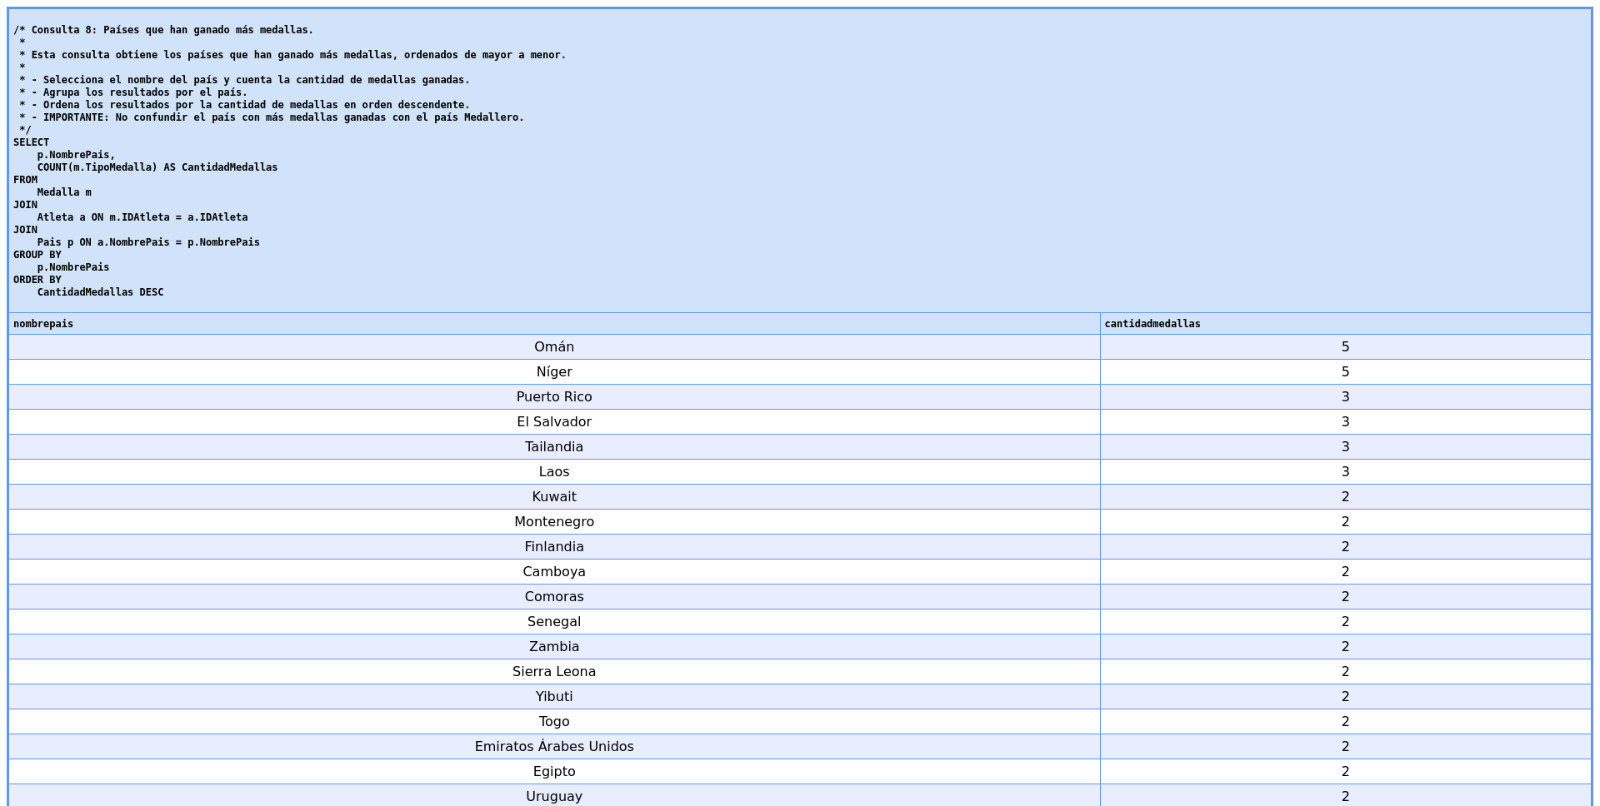
\includegraphics[width=16.5cm]{resources/Chapters/Consultas/Imagenes/Consulta8.jpg} 
	
	Consulta 8. Países que han ganado más medallas.
\end{center}

\textbf{Propósito de la consulta}

La consulta tiene como objetivo identificar los países que han ganado más medallas, mostrando su nombre y la cantidad de medallas ganadas, ordenados de mayor a menor. Esto permite observar el desempeño acumulado de los países en términos de logros deportivos.

\textbf{Desglose de la consulta}

\begin{itemize} \item \textbf{Selección de columnas (\texttt{SELECT}):} \begin{itemize} \item \texttt{p.NombrePais}: Muestra el nombre del país al que se asignan las medallas. \item \texttt{COUNT(m.TipoMedalla) AS CantidadMedallas}: Cuenta la cantidad total de medallas ganadas por cada país, independientemente del tipo (oro, plata o bronce). \end{itemize}
	
	\item \textbf{Tablas involucradas (\texttt{FROM} y \texttt{JOIN}):} \begin{itemize} \item \texttt{Medalla (m)}: Tabla que registra las medallas ganadas, incluyendo información sobre el atleta que las obtuvo. \item \texttt{Atleta (a)}: Tabla que relaciona a cada medalla con un atleta específico mediante la clave \texttt{m.IDAtleta = a.IDAtleta}. \item \texttt{Pais (p)}: Tabla que asocia cada atleta con su respectivo país mediante la relación \texttt{a.NombrePais = p.NombrePais}. \end{itemize}
	
	\item \textbf{Agrupación de resultados (\texttt{GROUP BY}):} \begin{itemize} \item La agrupación se realiza por \texttt{p.NombrePais}, permitiendo que las medallas se contabilicen para cada país de forma independiente. \end{itemize}
	
	\item \textbf{Ordenamiento de resultados (\texttt{ORDER BY}):} \begin{itemize} \item Los resultados se ordenan por la columna \texttt{CantidadMedallas} en orden descendente (\texttt{DESC}), para que los países con más medallas aparezcan primero. \end{itemize} \end{itemize}

\textbf{Análisis detallado}

\begin{itemize} \item \textbf{Relación entre tablas:} \begin{itemize} \item Existe una relación jerárquica que conecta \texttt{Medalla} con \texttt{Atleta} y \texttt{Atleta} con \texttt{Pais}: \begin{itemize} \item Cada medalla (\texttt{Medalla}) se asigna a un atleta específico (\texttt{Atleta}). \item Cada atleta pertenece a un país (\texttt{Pais}). \item Por lo tanto, las medallas de cada país se calculan mediante esta relación indirecta. \end{itemize} \end{itemize}
	
	\item \textbf{Uso de la función agregada \texttt{COUNT}:} \begin{itemize} \item La función \texttt{COUNT(m.TipoMedalla)} cuenta cuántas medallas (de cualquier tipo) están asociadas a cada país. \item Esto implica que no se diferencia entre tipos de medalla, sino que todas las medallas tienen el mismo peso en el conteo. \end{itemize}
	
	\item \textbf{Agrupación por país:} \begin{itemize} \item Agrupar los resultados por \texttt{p.NombrePais} asegura que las medallas se contabilicen de manera acumulativa para cada país. \end{itemize}
	
	\item \textbf{Ordenamiento por cantidad de medallas:} \begin{itemize} \item Ordenar los resultados por \texttt{CantidadMedallas} en orden descendente facilita la identificación de los países con mejor desempeño en términos de medallas ganadas. \end{itemize} \end{itemize}

\textbf{Posibles escenarios y consideraciones}

\begin{itemize} \item \textbf{Países sin medallas:} \begin{itemize} \item Los países sin medallas no aparecerán en los resultados, ya que la consulta utiliza la función \texttt{COUNT}, que excluye filas sin registros asociados. \end{itemize}
	
	\item \textbf{Medallas compartidas:} \begin{itemize} \item Si un sistema permite que una medalla sea compartida por varios atletas de diferentes países, la consulta no maneja este caso explícitamente. \end{itemize}
	
	\item \textbf{Empates en el conteo:} \begin{itemize} \item Si dos países tienen la misma cantidad de medallas, el orden relativo entre ellos no está definido, pero esto no afecta el propósito principal de la consulta. \end{itemize} \end{itemize}

Esta consulta es útil para analizar el desempeño de cada país en términos de medallas ganadas, proporcionando información valiosa para comparaciones y estudios de rendimiento deportivo.